\documentclass[12pt]{article}
\usepackage[english]{babel}
\usepackage{t1enc}
\usepackage{geometry}
\usepackage{graphicx}
\usepackage{float}
\usepackage{caption}
\usepackage{amsmath,amsthm,amsfonts,amssymb,amscd}
\usepackage{hyperref}
\usepackage{fancyhdr}
\usepackage{nicefrac}
\usepackage{titlesec}
\usepackage{pdfpages}
\usepackage{mathtools}
\usepackage{siunitx}
\usepackage{pdflscape}
\usepackage{csquotes}


\geometry{
a4paper,
total={170mm,240mm},
left=20mm,
top=30mm,
}

\pagestyle{empty}
\date{}

\pagestyle{fancyplain}
\headheight 35pt
\rhead{\Course}
\chead{\textbf{\Large \Title}}
\lhead{\Date }
\lfoot{}
\cfoot{}
\rfoot{\small\thepage}
\headsep 1.5em


\renewcommand{\d}[1]{\mathrm{d}#1}

\sisetup{exponent-product = \cdot,
         output-product = \cdot,
         per-mode=fraction}


\usepackage[backend=biber,style=numeric,sorting=none]{biblatex}

\addbibresource{parts/literature.bib}

\newcommand{\specialcell}[2][c]{\begin{tabular}[#1]{c}#2\end{tabular}}


%Define those, after that everything is nice and automatic
\newcommand\Title{Group Assignment}
\newcommand\Date{\today}
\newcommand\Name{Ádám Kohajda \\ Dániel Nagy \\ József Szenka \\ László Kocsis \\ Zoltán Hafner}
\newcommand\Course{Marketing}
\newcommand\Neptun{BMEGT20MW01}
\newcommand\CourseNeptun{BMEGT20MW01}

\begin{document}


\frenchspacing
\thispagestyle{empty} %Ne legyen header

\begin{center}
\Large{\Course} \\
\vskip 0.25cm
\large{\CourseNeptun}
\vskip 2cm

\huge{\Title}

\vskip 2cm
\Huge{\textbf{German beers to Hungarian market (webshop)}}

\vskip 3cm
\Large{\Name}\\

\mbox{}
\vfill

\begin{figure}[htb]
   \centering
   
\includegraphics[width=0.7\linewidth]{pics/bme-logo.jpg}
\end{figure}


\large{Budapest University of Technology and Economics} \\
\large{Budapest, 2022}


\pagebreak
\setcounter{page}{1}

\end{center}
 %sometimes include only a pdf instead
%\includepdf[pages=-]{parts/task.pdf} %replace this page
\tableofcontents



\section{Introduction}
What is the first thing that comes to Your mind, when it comes to Germany? Is it their world-renowned technological achievements, or their spicy cuisine? Whatever it may be, there is no single soul, that has not heard about their famous beer culture.

Germans are one of the largest beer consumers in Europe. According to studies an average German consumes around 140 litres of beer annually. However, they do not only like to drink beer, but also brew it. It is estimated that there are currently around 1300 operating breweries in Germany, that produce more than 110 hectolitre beer every year \cite{statista1}. In order to maintain German beer quality, there is a German Purity Law, which controls the allowed ingredients of a beer. According to the statue may only use malt, hops, yeast and water to brew beer.

With all this in mind, we decided to bring a “sip” of the German beer culture to Hungary. Our mission is to make the century old beer selections available to the Hungarian market. Currently there are only a handful of accessible German beers to the Hungarian consumers. That’s why we would like to broaden the German beer selection. Our solution includes a webshop, through which consumers can order dozens of different German beers.

The domestic beer market has undergone a dynamic transformation in the recent years. As a result, more and more craft breweries are present in Hungary. We want to ride this trend and promote German beers among Hungarian consumers.

\newpage
\section{Analysis}
\subsection{Market segmentation}

\begin{itemize}
   \item Geographic segmentation is relevant to our marketing plan. Our main target is Hungary and, more precisely, the capital and large cities, these cities can be seen in Fig. \ref{fig:hu}. People living in rural areas and smaller towns are less likely to buy our products as they tend to have less disposable income. This segment also uses the internet less and prefers offline shopping. On the other hand, inhabitants of larger cities tend to be more prosperous and more active online. According to the Hungarian Central Statistical Office, the size of this geographic segment consists of 3.6 million people and is also growing. \cite{ksh1}

   \item Demographic segmentation is also essential to take into account in our case. The more vital sub-categories to consider are age, life-cycle stage, income and gender. According to the Hungarian Central Statistical Office (source), the most significant beer drinkers are mature, aged between 30-60 years men. \cite{ksh2} If we examine beer consumption habits in Hungary, men consume more than twice the amount of beer as women and can be shown male surplus in this age range. We target this specific segment of society. This product of ours represents the higher cost quality beers, so it demands purchasing power. Thus the younger cannot afford it frequently, but the middle-aged with a stable income can be recurring customers. Other aspects of demographic segmentation, like occupation, education, religion and ethnicity in our target, are not necessary because these do not show significant consumption differences.


   \item Under psychographic and behavioral segmentation we state that our main targets are men from the middle and upper class, who are seeking for diverse high quality beers, and how can afford it. In there lifestyle they consume these product rarely (once or twice a week) but on greater occasions many of them together with there friends.
\end{itemize}

\begin{figure}[H]
  \centering
  \begin{subfigure}[t]{0.45\textwidth}
  	\centering
  	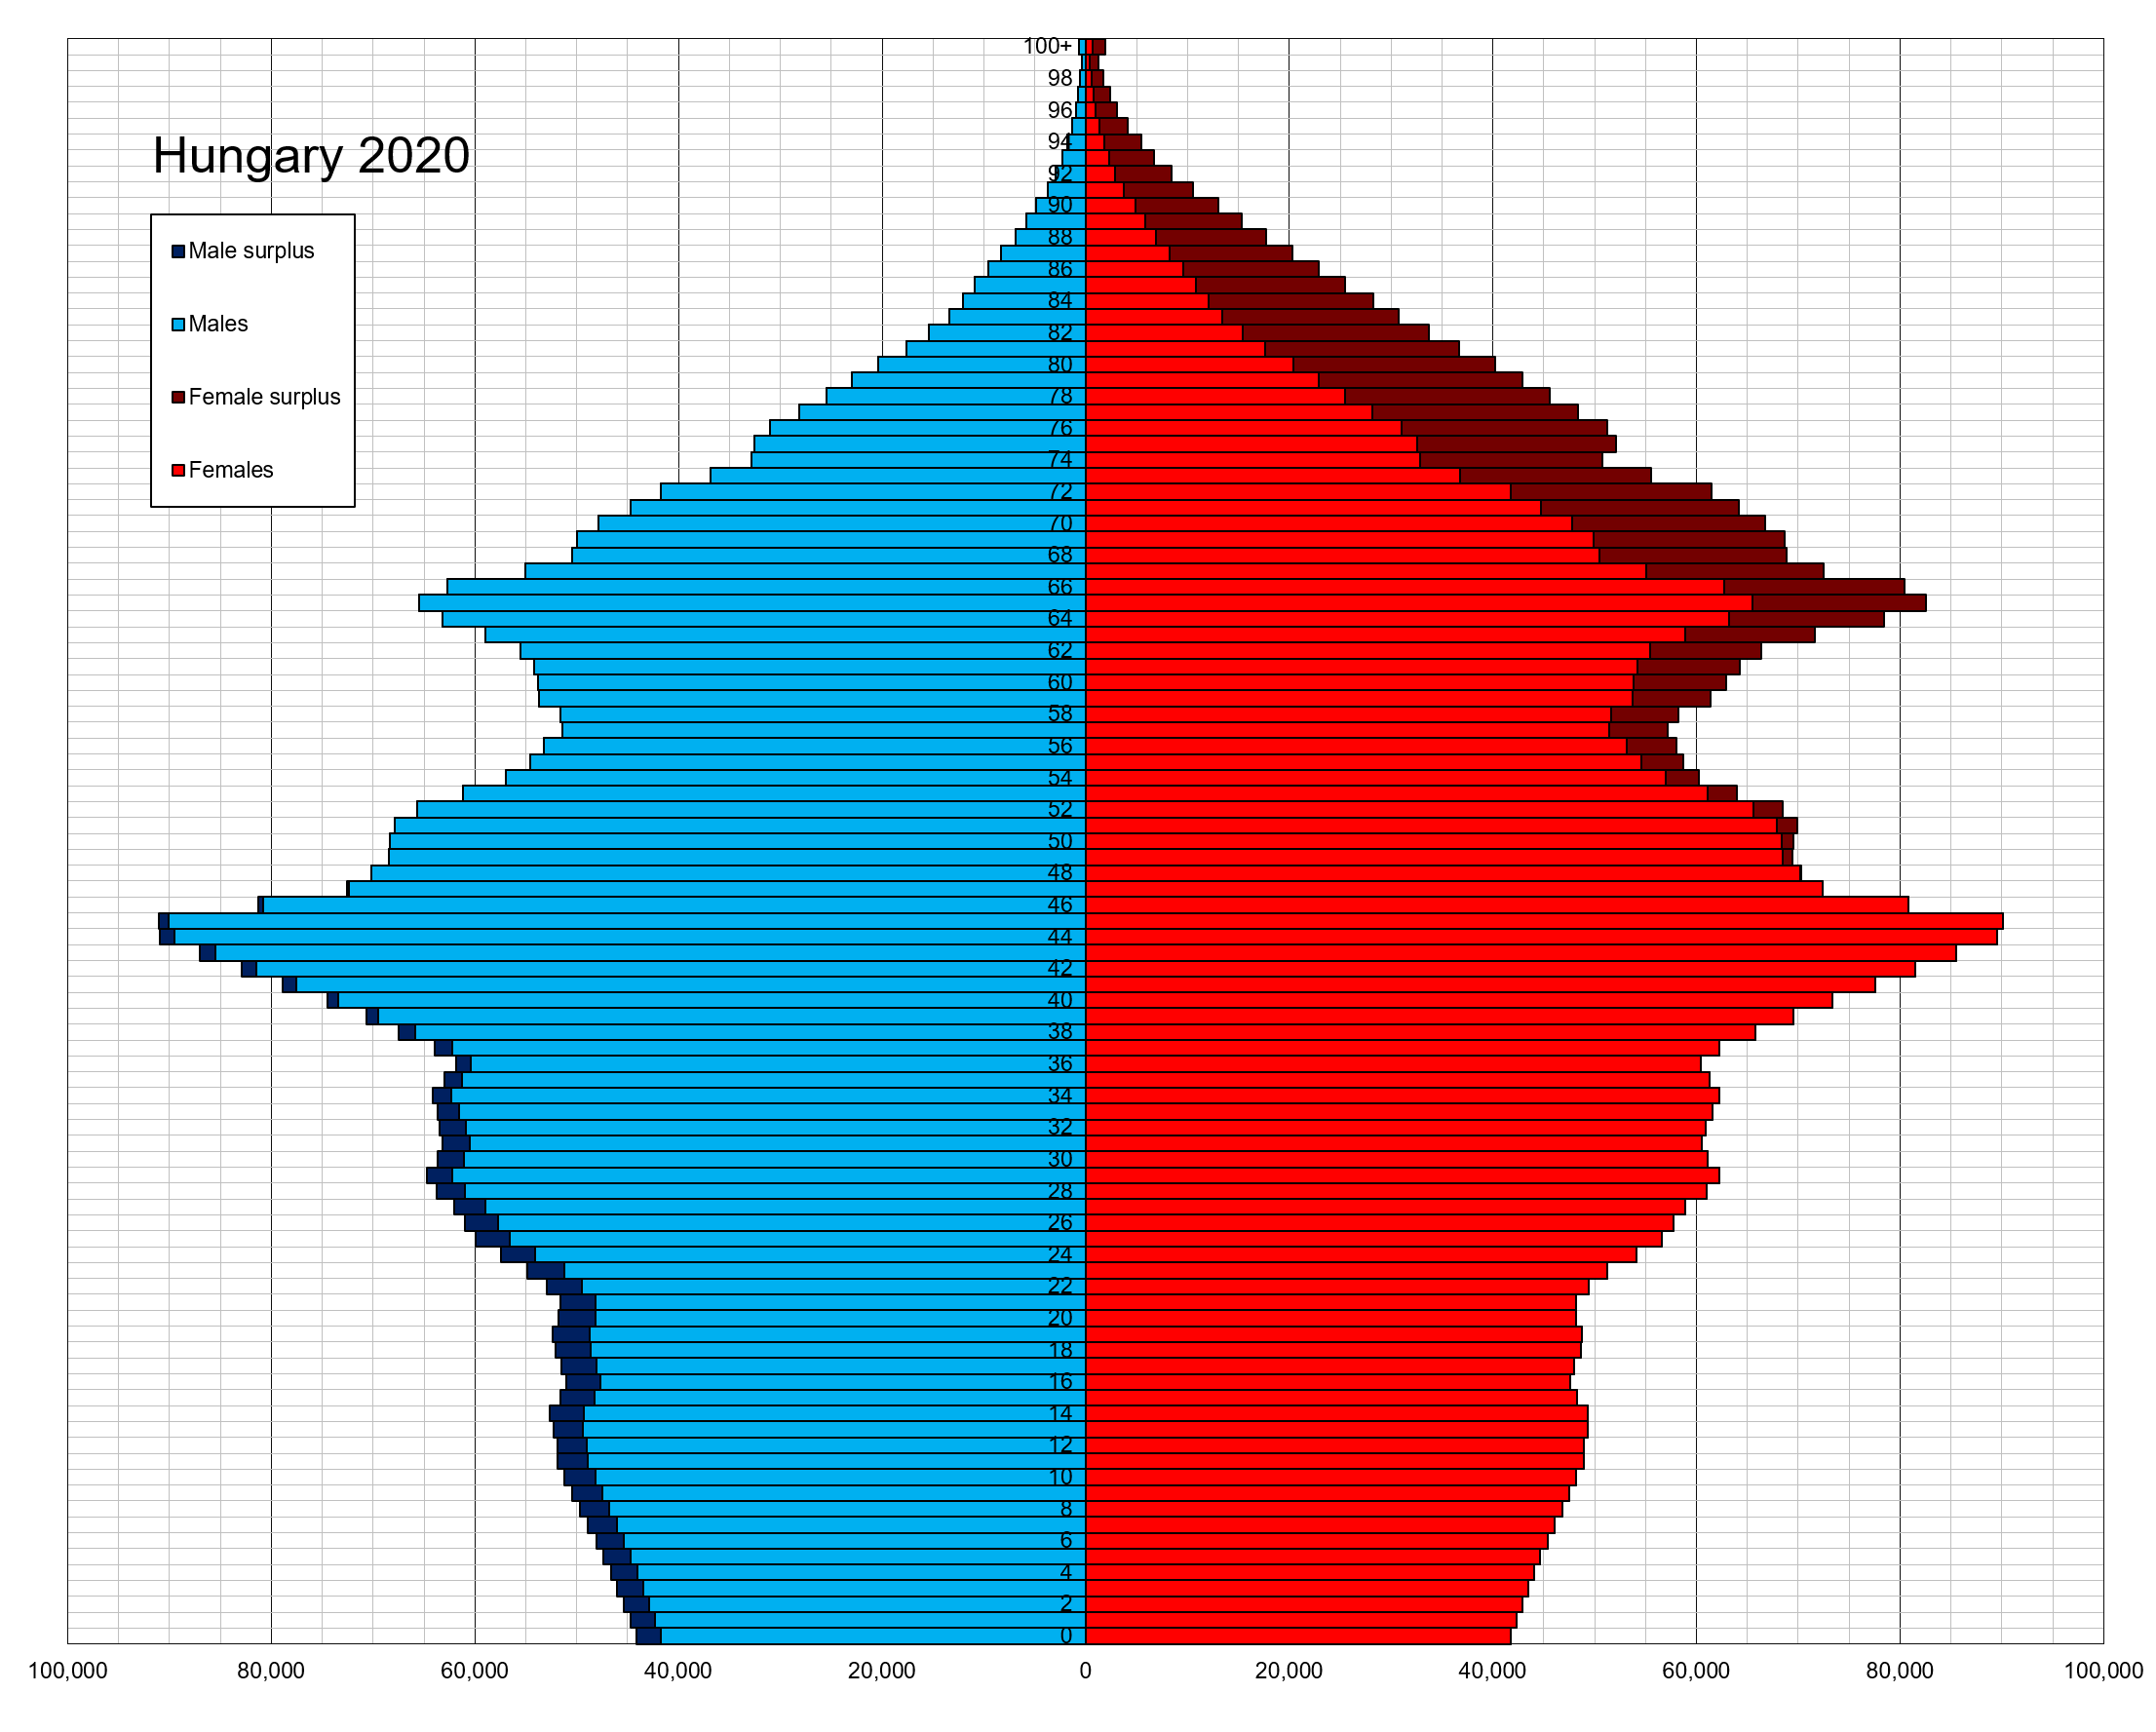
\includegraphics[width=0.8\linewidth]{pics/hungary.png}
  	\caption{Population pyramid of Hungary \cite{wiki1}}
  \end{subfigure}
  \begin{subfigure}[t]{0.45\textwidth}
  	\centering
  	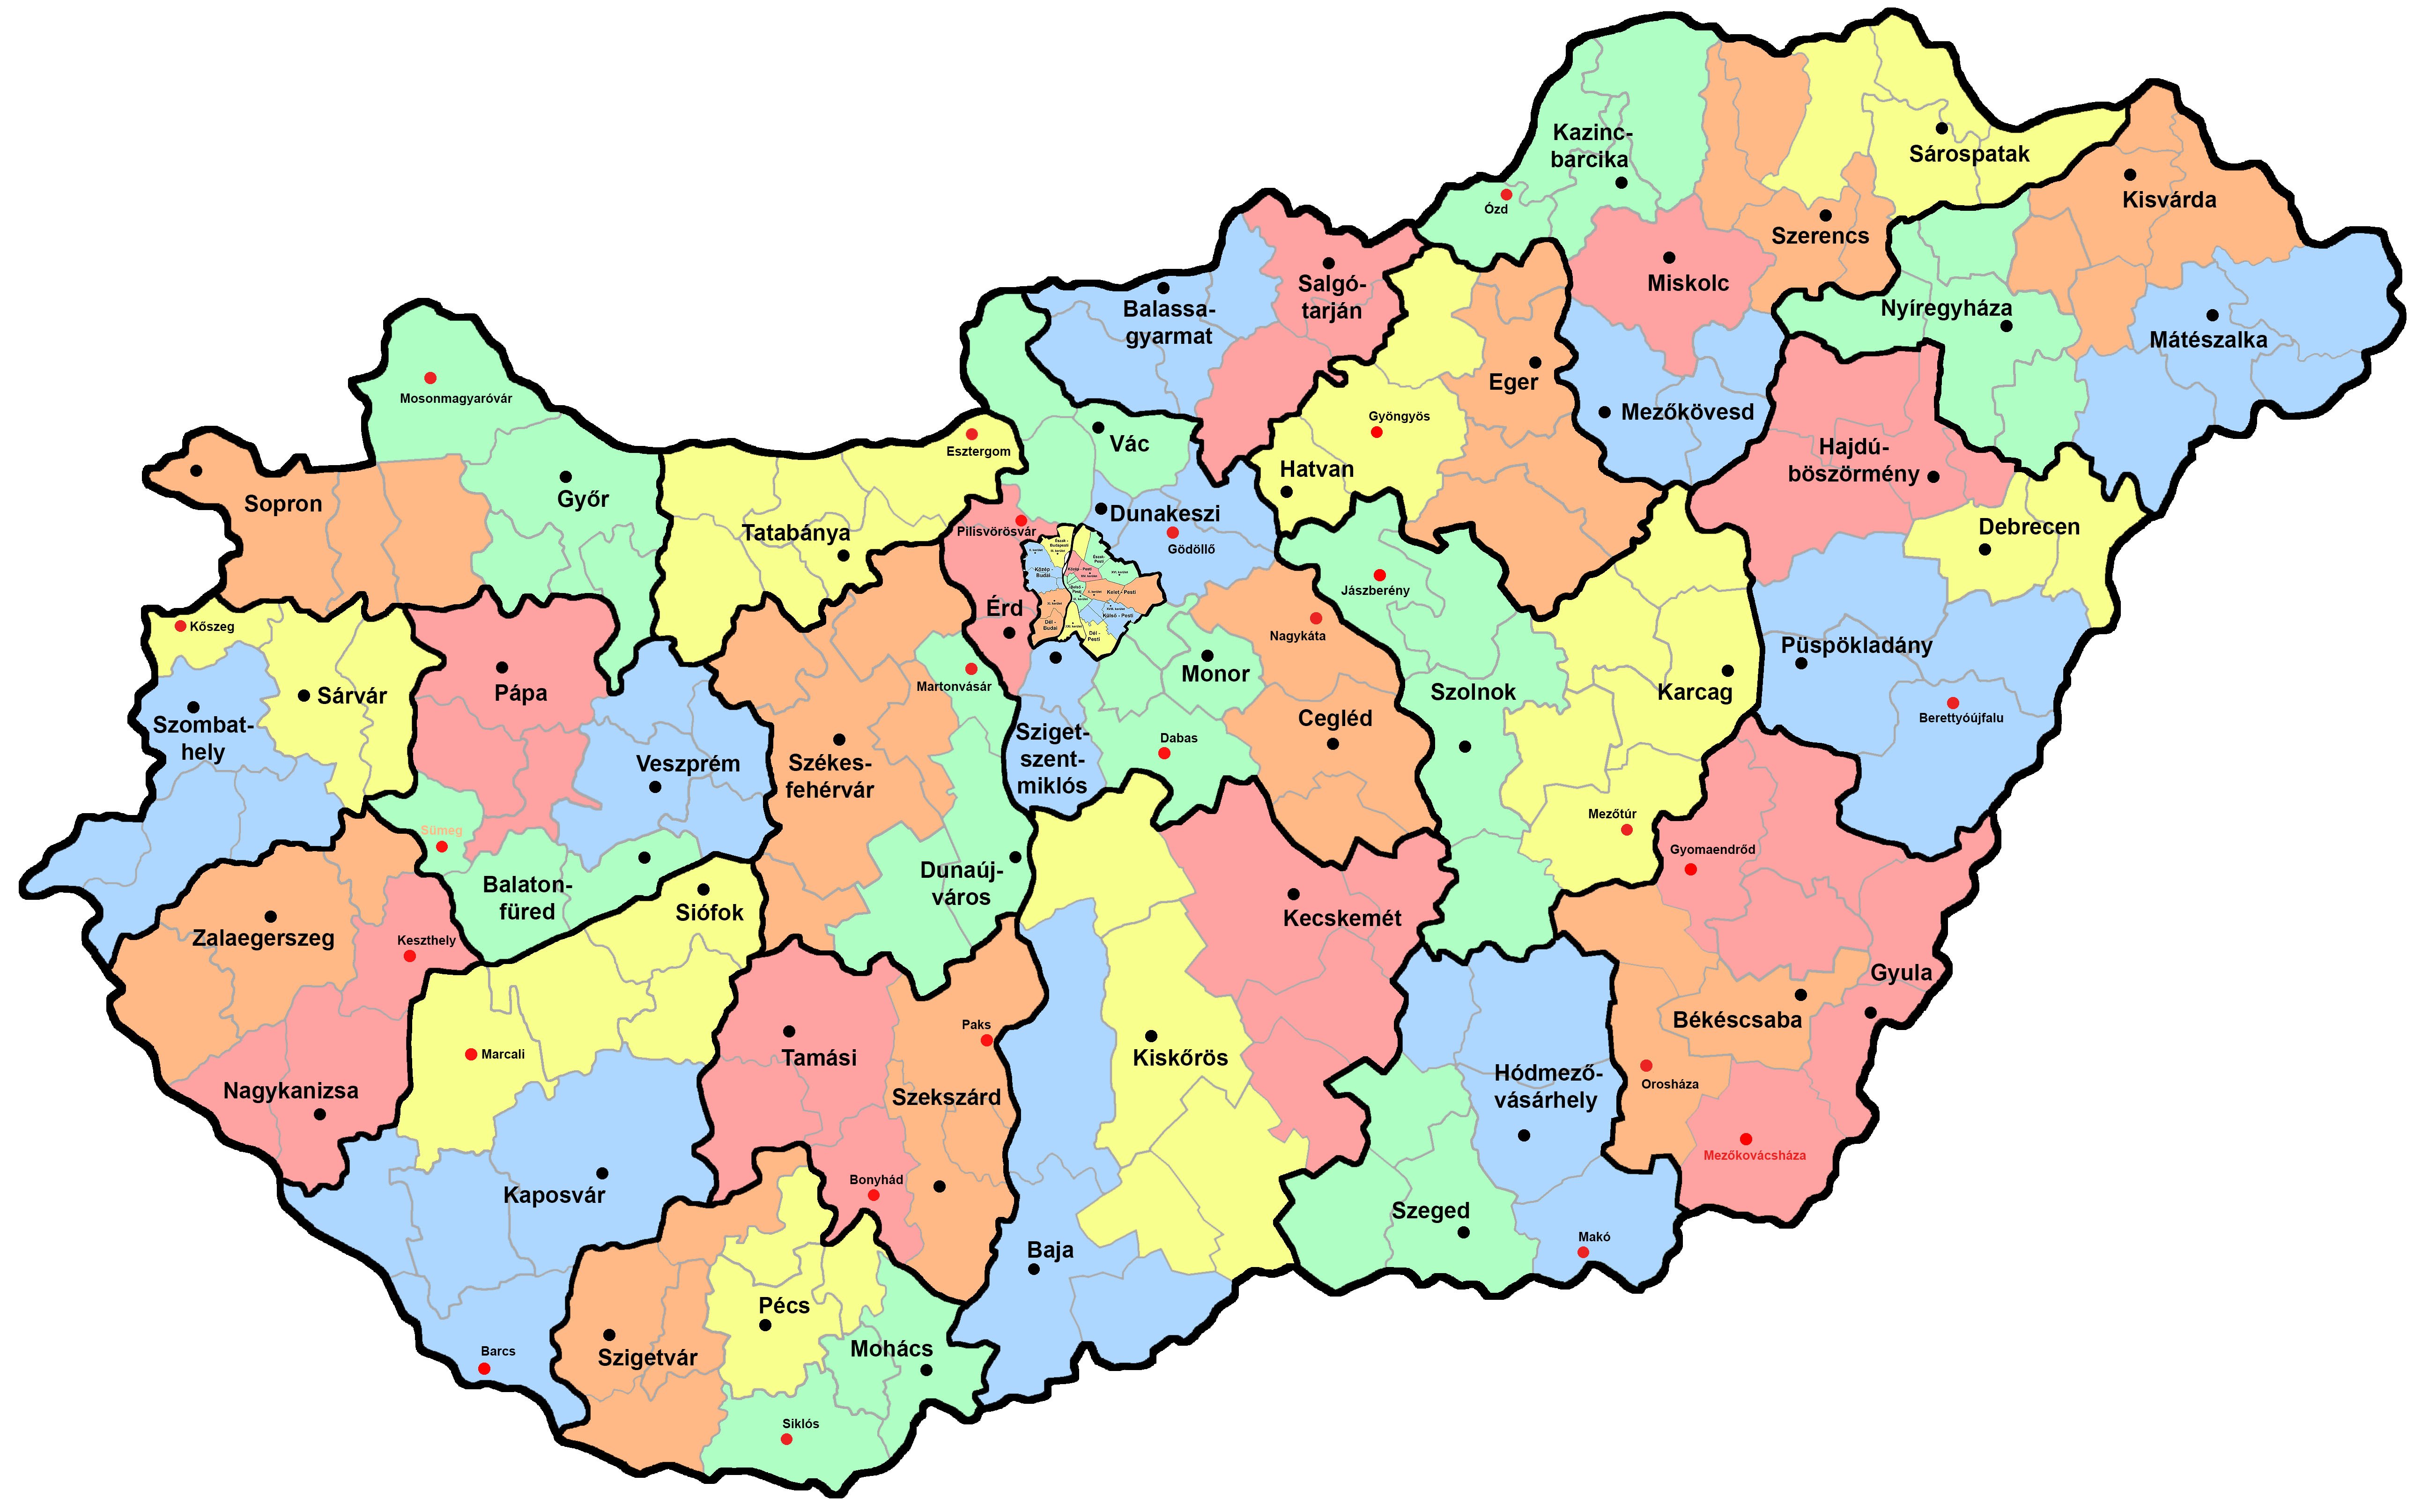
\includegraphics[width=\linewidth]{pics/magyar.jpg}
  	\caption{\centering The map of Hungarian larger cities \cite{terkep}}
  \end{subfigure}
  \caption{The  project related Hungarian data}
  \label{fig:hu}
\end{figure}

\subsection{Market targeting}

\subsubsection*{Which segment to target?}

Our company targets a well defined market segment. This segment is stable by purchasing power, fast growth or reduction is not expected. Nevertheless it worth to mention that the segment is getting more and more open to imported beers, thus the market is growing rapidly. According the data of KSH (see Fig. \ref{fig:ksh} and \cite{ksh2}) the amount of imported beers to the Hungarian market grew by 64.5\% between 2017 and 2019.


\subsubsection*{How to target them?}

The targeting strategy of the company is focusing on the defined market segment. This concentrated marketing is a big advantage for our new business. It is very efficient and effective. We can collect data about the habits and not satisfied demands through several research methods.
Focus group is a good option with sample products. During these research events the costumers can get familiar with our products and in the same time they provide very helpful feedbacks to the company. To reach more people it is an obvious solution for a webstore company that the main platform of the marketing is online. According online surveys the company can optimize the distribution of beers types, we are offering.


\subsection{Market positioning}


Our positioning strategy is based on the following value proposition:  \textit{more for more}. It means that we provide a better customer experience (e.g. faster shipping, better quality) than our competitors, however we also request a higher price for this. A creative approach should be taken to rationalise correlated advertising material. Our positioning statement reflects just that:

\textit{To quality beer consumers who enjoy a wide variety of German beers, our webshop is the ultimate place that delivers the perfect beer for your every day consumption as well as for special occasions.}



Our main competitors are listed below. The common factor of our competitors is that they do not specialize in German beers.
\begin{itemize}
   \item \texttt{soronline.hu} \cite{soronline}
   \item \texttt{beerselection.hu} \cite{beerselection}
   \item \texttt{beergourmet.hu} \cite{beergourmet}
   \item \texttt{csakajosor.hu} \cite{csakajosor}
\end{itemize}
Compared to other webshops importing and distributing foreign beer selections, we would like to first limit our import products to the German market. Therefore, we can bring a greater variety of German beers to our intended customers. Because all our competitors focus on worldwide beer selections, they can only offer a few German beer types, thus not enabling to fully experience the German beer culture. As stated before, we would like to prioritise German beer types and thanks to the hundreds of different German breweries we can broaden the selection.

In our communication it is important to emphasize the high quality and the diversity of our product assortment. Related to this since we are distributing only German beers, we have a better connection to the factories, we can deliver special products that are not available elsewhere.


\section{Summary}
Our main finding is that we should focus our marketing strategy on middle aged men living in larger Hungarian cities. This group of people has the wealth and the demand to buy better quality products. That way our service can reach to many people who is looking for these product and they can be easily satisfied with our proficiency and excellent costumer support. Alongside that we can be sure that the need for this service and these products will increase, while the quality of life in Hungary also increases, and that way our service can expand and reach to more and more people. 


\newpage
\renewcommand{\baselinestretch}{1}

\newpage

\printbibliography
 %comment it out if not needed
\addcontentsline{toc}{section}{References}

\section*{Appendix}
\addcontentsline{toc}{section}{Appendix}
\begin{figure}[H]
  \centering
  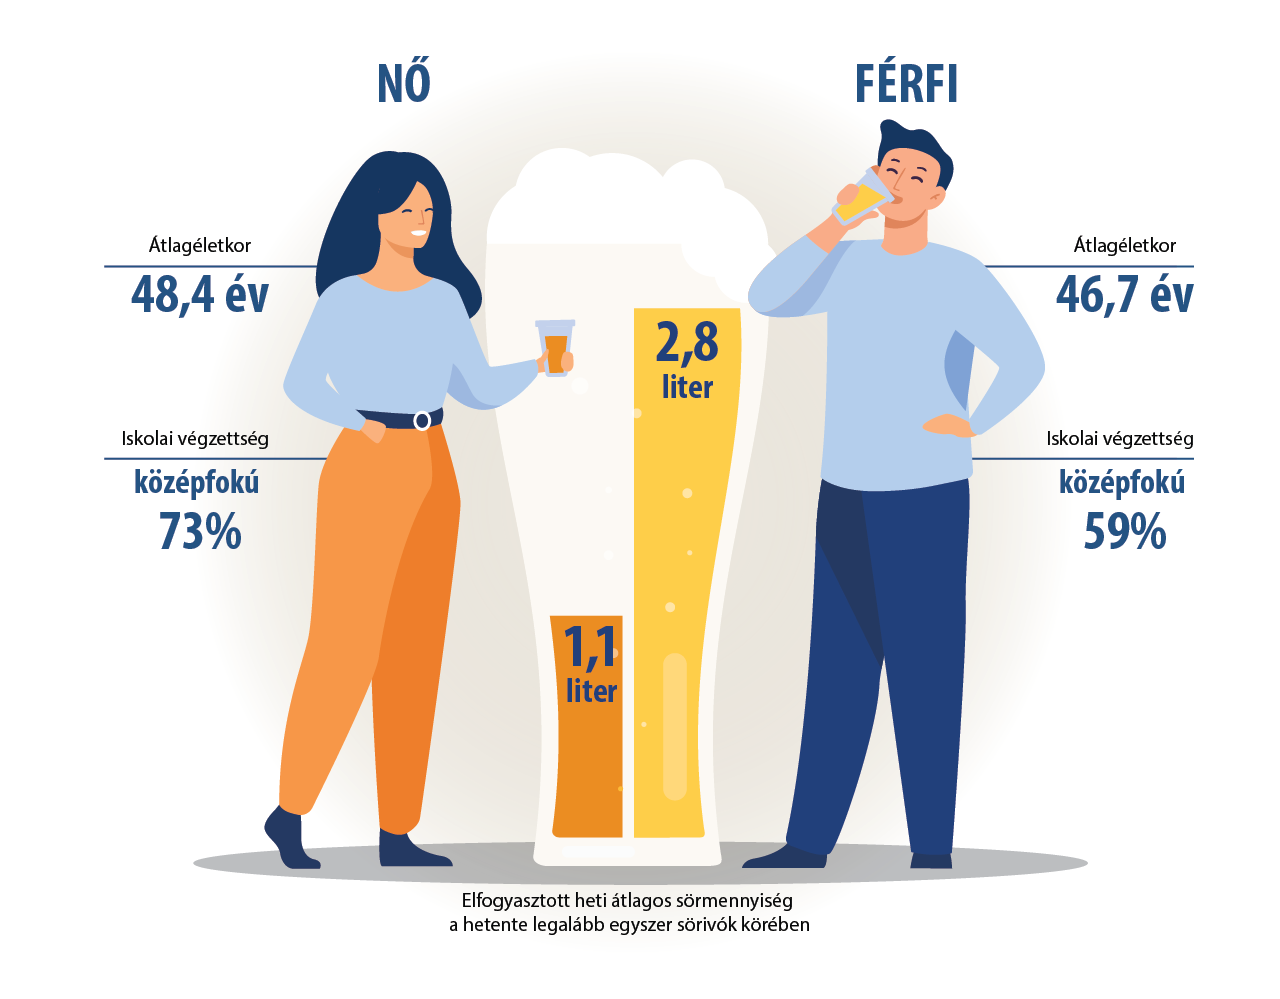
\includegraphics[width=0.65\linewidth]{pics/ksh.png}
  \caption{Beer consumption behaviour of men and women in Hungary \cite{ksh2}}
  \label{fig:ksh}
\end{figure}

\end{document}
